\documentclass{article}
\usepackage[utf8]{inputenc}
\usepackage[english]{babel}

\usepackage{graphicx}
\usepackage{hyperref}
\hypersetup{
    colorlinks=true,
    linkcolor=blue,
    filecolor=magenta,      
    urlcolor=cyan,
}

\begin{document}

\section{Introduction} % (fold)
\label{sec:introduction}



% section introduction (end)https://commons.wikimedia.org/wiki/File:Martin-Dougiamas.jpg#/media/File:Martin-Dougiamas.jpg


\subsection{Web Presence} % (fold)
\label{sub:web_presence}

% subsection web_presence (end)
% section history (end)

\section{History} % (fold)
\label{sec:history}

Moodle is an open-source learning management system. It is written in PHP, JavaScript and using SQL as the database \footnote{http://}. It was devleoped by Martin Dougiamas as a part of his PhD thesis research. Dougiamas started developing the initial version of Moodle in 1999 out of his desperation of using the available commercial software. Since then, the size and activities within the project have grown substantially.

\begin{figure}[h!]
	\centering
	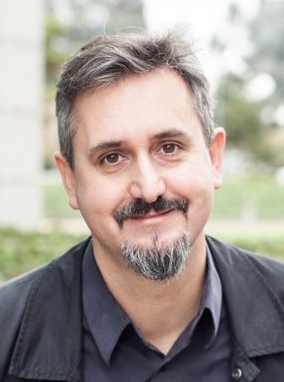
\includegraphics[scale=0.5]{Martin-Dougiamas.jpg}
	\label{fig:martin}
	\caption{Martin Dougiamas (Source: Dougiamas (Own Work) [\href{http://creativecommons.org/licenses/by-sa/4.0}{CC BY-SA 4.0}],
	\href{https://commons.wikimedia.org/wiki/File\%3AMartin-Dougiamas.jpg}{via Wikimedia Commons})}
\end{figure}



\subsection{Releases} % (fold)
\label{sub:releases}

% subsection releases (end)

% section history (end)

\section{Who develops Moodle?} % (fold)
\label{sec:who_develops_moodle_}

\subsection{Location} % (fold)
\label{sub:location}

% subsection location (end)

\subsection{Lead Developers} % (fold)
\label{sub:lead_developers}

% subsection lead_developers (end)
% section who_develops_moodle_ (end)

\section{Governance} % (fold)
\label{sec:governance}

\subsection{Project Team} % (fold)
\label{sub:project_team}

% subsection project_team (end)

\subsection{Copyright} % (fold)
\label{sub:copyright}

% subsection copyright (end)

\subsection{Legal} % (fold)
\label{sub:legal}

% subsection legal (end)

\subsection{Finances} % (fold)
\label{sub:finances}

% subsection finances (end)

% section governance (end)

\section{Licensing} % (fold)
\label{sec:licensing}

% section licensing (end)

\section{Culture} % (fold)
\label{sec:culture}

% section culture (end)


\section{Relationships with other projects} % (fold)
\label{sec:relationships_with_other_projects}

% section relationships_with_other_projects (end)

\section{Source code management} % (fold)
\label{sec:source_code_management}

% section source_code_management (end)

\section{Documentation} % (fold)
\label{sec:documentation}

% section documentation (end)

\section{Bug tracking and support} % (fold)
\label{sec:bug_tracking_and_support}

\subsection{Support} % (fold)
\label{sub:support}

% subsection support (end)

\subsection{IRC} % (fold)
\label{sub:irc}

% subsection irc (end)

\subsection{Bug Tracker} % (fold)
\label{sub:bug_tracker}

% subsection bug_tracker (end)

\subsection{Forums} % (fold)
\label{sub:forums}

% subsection forums (end)

\subsection{Mailing List} % (fold)
\label{sub:mailing_list}

% subsection mailing_list (end)

% section bug_tracking_and_support (end)

\section{How are releases managed} % (fold)
\label{sec:how_are_releases_managed}

% section how_are_releases_managed (end)

\section{Future development} % (fold)
\label{sec:future_development}

% section future_development (end)

\section{Summary} % (fold)
\label{sec:summary}

% section summary (end)
\end{document}